\chapter{Kromatografi}\label{ch:b2:chromatography}

Setetes minuman energi, yang diencerkan dan disaring, disuntikkan ke dalam
tabung baja yang tidak lebih panjang daripada sebatang pena dan diisi
butiran silika berukuran beberapa mikrometer. Beberapa menit kemudian
sebuah detektor telah menggambar garis dengan segelintir puncak, dan dari
luas salah satunya laboratorium melaporkan berapa banyak kafeina yang ada
dalam kaleng itu, dengan ketelitian beberapa persen. \omterm{def:b2:chromatography:principle}{Kromatografi} memisahkan
komponen-komponen sebuah campuran dengan membiarkannya berlomba melalui
sebuah kolom dengan kecepatan yang berbeda-beda; bab ini menjelaskan mengapa
kecepatannya berbeda, mengapa puncak-puncaknya mempunyai lebar seperti itu,
bagaimana memisahkan dua tetangga, dan bagaimana mengubah sebuah puncak
menjadi sebuah kuantitas.

\begin{omfigure}
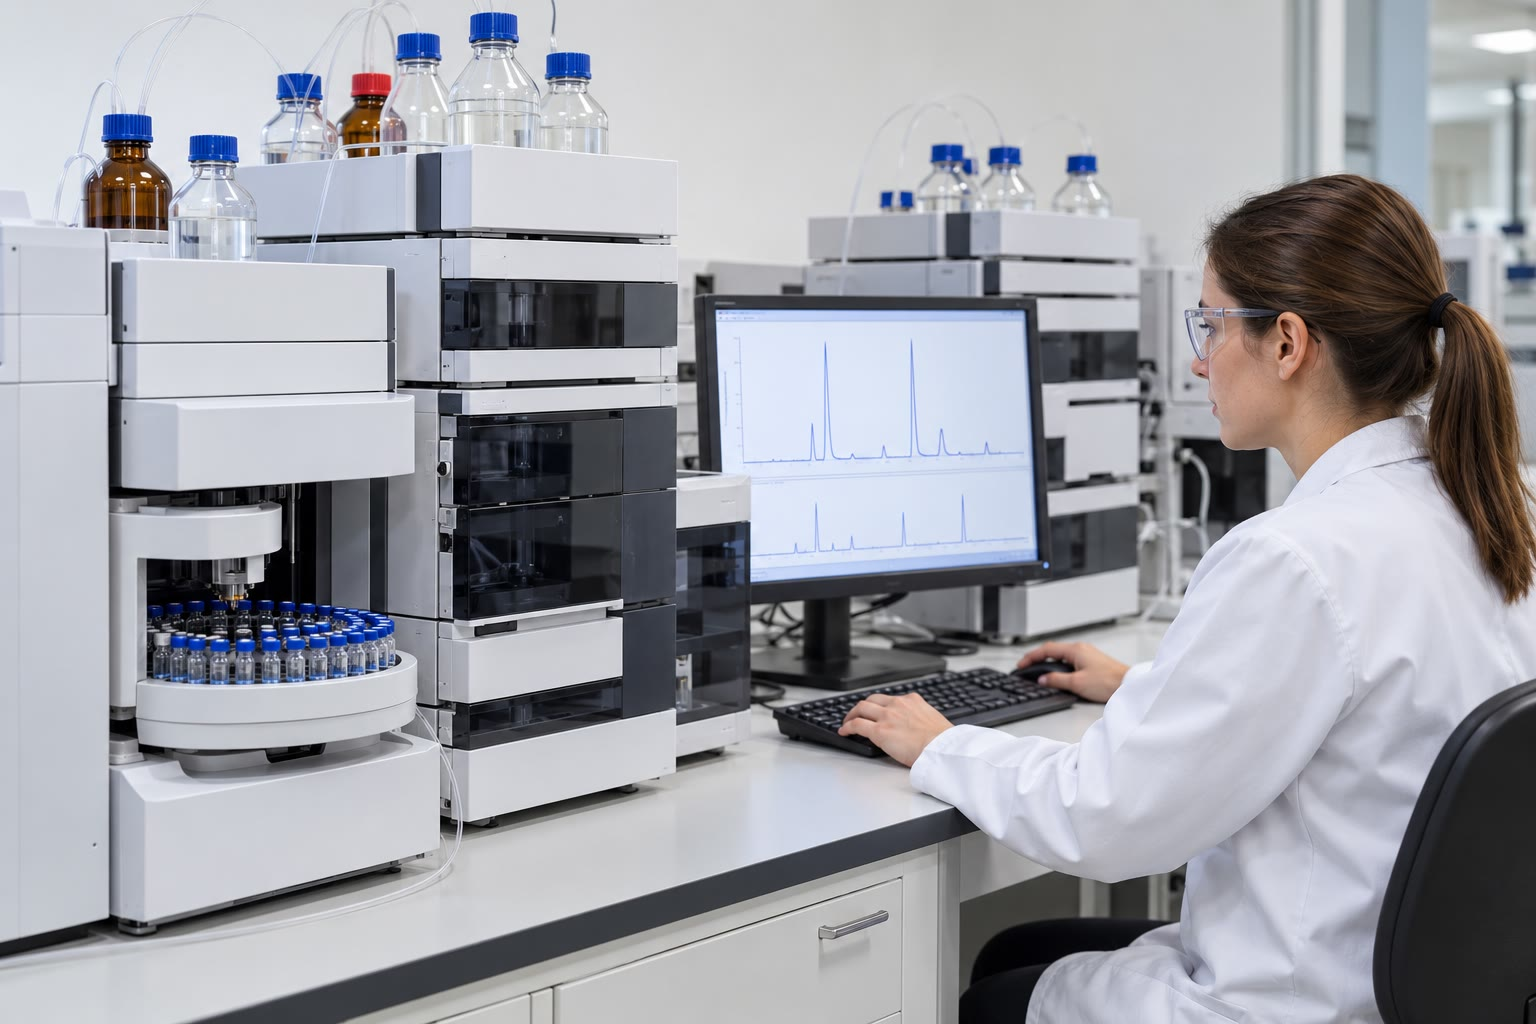
\includegraphics[width=0.58\linewidth]{images/book3/ai/b2-31-analytical-lab.jpg}

{\small Sebuah laboratorium analitik: kromatograf cair dengan botol-botol
pelarutnya dan baki vial pengambil sampel otomatis; kromatogram muncul di
layar (ilustrasi).}
\end{omfigure}

\begin{recall}
Jilid sekolah: \omterm{def:b2:chromatography:principle}{kromatografi} kertas dan lapis tipis, kromatogram, eluen.
Jilid Tahun 1: koefisien partisi, ekstraksi cair--cair, \omterm{def:b2:chromatography:retention}{faktor retensi}
$R_f$ pelat lapis tipis.
\Cref{ch:b2:liquid-vapour-diagrams}: \omterm{def:b2:liquid-vapour-diagrams:fractional-distillation}{pelat teoretis} kolom distilasi.
\end{recall}

\section{Prinsip}

\begin{definition}[Kromatografi]\label{def:b2:chromatography:principle}
Yang disebut \emph{kromatografi}\index{kromatografi} memisahkan
komponen-komponen sebuah campuran dengan mendistribusikannya di antara
\emph{fase diam}\index{fase diam}, yang terpasang tetap di dalam kolom atau
pada pelat, dan \emph{fase gerak}\index{fase gerak}, yaitu gas atau cairan
yang mengalir melewatinya. Membawa komponen-komponen itu melalui dan keluar
dari kolom bersama fase gerak disebut \emph{elusi}\index{elusi}.
\end{definition}

Sebuah molekul hanya bergerak selama berada dalam \omterm{def:b2:chromatography:principle}{fase gerak}; selama
ditahan oleh \omterm{def:b2:chromatography:principle}{fase diam}, molekul itu menunggu. Molekul itu berpindah di
antara kedua fase jutaan kali dalam perjalanannya, sehingga kecepatan
rata-ratanya ditentukan oleh fraksi waktu yang dihabiskannya dalam
masing-masing fase, yaitu oleh kesetimbangan partisinya.

\begin{definition}[Retensi]\label{def:b2:chromatography:retention}
Yang disebut \emph{waktu retensi}\index{waktu retensi} $t_R$ sebuah senyawa
adalah waktu dari penyuntikan sampai maksimum puncaknya; \emph{waktu
mati}\index{waktu mati} $t_M$ adalah waktu retensi senyawa yang tidak
tertahan, yang tidak pernah masuk ke \omterm{def:b2:chromatography:principle}{fase diam}. Yang disebut \emph{faktor retensi}\index{faktor retensi k@faktor retensi $k$}
$k$ sebuah senyawa pada sebuah kolom adalah
\begin{equation*}
k = \frac{t_R - t_M}{t_M}.
\end{equation*}
Faktor ini bukan $R_f$ pelat lapis tipis, yang mengukur jarak yang
ditempuh, walaupun keduanya menggambarkan partisi yang sama.
\end{definition}

\begin{proposition}[Waktu retensi]\label{prop:b2:chromatography:retention-time}
Jika, pada kesetimbangan, jumlah sebuah senyawa dalam \omterm{def:b2:chromatography:principle}{fase diam} dan \omterm{def:b2:chromatography:principle}{fase
gerak} sebuah irisan kolom adalah $n_s$ dan $n_m$, senyawa itu bergerak
dengan kecepatan $u/(1 + n_s/n_m)$, dengan $u$ kecepatan \omterm{def:b2:chromatography:principle}{fase gerak},
dan $t_R = t_M(1 + n_s/n_m)$.
\end{proposition}

\begin{proof}
Sebuah molekul tertentu menghabiskan fraksi $n_m/(n_s + n_m)$ waktunya
dalam \omterm{def:b2:chromatography:principle}{fase gerak}, tempat molekul itu bergerak dengan kecepatan
$u$, dan sisanya diam. Kecepatan rata-ratanya adalah $u\,n_m/(n_s + n_m) = u/(1 + n_s/n_m)$.
Kolom sepanjang
$L$ dilintasi dalam waktu $t_R = (L/u)(1 + n_s/n_m)$, dan $L/u = t_M$.
\end{proof}

\begin{proposition}[Retensi dan partisi]\label{prop:b2:chromatography:k-and-K}
\omterm{def:b2:chromatography:retention}{Faktor retensi} adalah rasio jumlah zat dalam kedua fase, $k = n_s/n_m = KV_s/V_m$, dengan $K$
koefisien partisi (konsentrasi dalam \omterm{def:b2:chromatography:principle}{fase diam} dibagi konsentrasi dalam
\omterm{def:b2:chromatography:principle}{fase gerak}) dan $V_s$, $V_m$ volume kedua fase di dalam kolom.
\end{proposition}

\begin{proof}
Dari \cref{prop:b2:chromatography:retention-time}, $(t_R - t_M)/t_M = n_s/n_m$. Dengan $n_s = c_sV_s$,
$n_m = c_mV_m$, dan $K = c_s/c_m$, $n_s/n_m = KV_s/V_m$.
\end{proof}

Dua senyawa terpisah jika koefisien partisinya berbeda; geometri kolom
($V_s/V_m$) mengalikan semua retensi secara sama. Mengubah \omterm{def:b2:chromatography:principle}{fase gerak}, yang
mengubah $K$, adalah tuas utama kimiawan untuk mengatur retensi.

\begin{omfigure}
\begin{tikzpicture}[x=1cm, y=1cm]
\foreach \x/\a/\b/\ha/\hb/\lab in {0/0.6/0.6/0.1/0.1/awal, 2.4/1.5/2.6/0.16/0.22/kemudian, 4.8/2.4/4.4/0.2/0.3/akhir}{
  \draw[black!60] (\x-0.35,0) rectangle (\x+0.35,-5);
  \fill[omThm!55] (\x-0.33,-\b+\hb) rectangle (\x+0.33,-\b-\hb);
  \fill[omDef!55, opacity=0.85] (\x-0.33,-\a+\ha) rectangle (\x+0.33,-\a-\ha);
  \node[font=\small] at (\x,-5.4) {\lab};
}
\draw[->, thick] (-1.0,-0.3) -- (-1.0,-4.6) node[midway, left, font=\small, align=right] {fase\\gerak};
\node[font=\small, align=left, anchor=west] at (5.5,-2.4) {lebih tertahan\\(lambat, sempit)};
\node[font=\small, align=left, anchor=west] at (5.5,-4.4) {kurang tertahan\\(cepat)};
\draw[densely dotted] (5.15,-2.4) -- (5.5,-2.4); \draw[densely dotted] (5.15,-4.4) -- (5.5,-4.4);
\end{tikzpicture}
\par\vspace{4pt}

{\small Dua senyawa yang disuntikkan bersama sebagai satu pita tipis bergerak
turun di dalam sebuah kolom (tiga potret sesaat, skematis). Senyawa yang
kurang tertahan ($k$ lebih kecil) berlari di depan; kedua pita melebar
selama bergerak, makin lebar pita yang telah menempuh jarak lebih jauh.}
\end{omfigure}

\section{Lebar puncak dan bilangan pelat}

Sebuah pita tidak tetap tipis. Molekul-molekul senyawa yang sama menempuh
jalur yang berbeda-beda di antara butiran, berdifusi sepanjang kolom, dan
tertinggal di \omterm{def:b2:chromatography:principle}{fase diam} dalam jumlah yang acak. Puncak yang tercatat di
ujung keluar hampir tepat berupa Gaussian dengan simpangan baku $\sigma_t$
(dalam waktu), dan makin sempit puncak itu untuk $t_R$ tertentu, makin baik
kolomnya.

\begin{definition}[Bilangan pelat]\label{def:b2:chromatography:plates}
Yang disebut \emph{bilangan pelat}\index{bilangan pelat} sebuah kolom untuk
sebuah senyawa adalah $N = (t_R/\sigma_t)^2$, dengan
$\sigma_t$ simpangan baku puncaknya dalam waktu. Yang disebut \emph{tinggi
pelat}\index{tinggi pelat} adalah
$H = L/N$, untuk kolom sepanjang $L$.
\end{definition}

Nama-nama itu berasal dari kolom distilasi pada \cref{ch:b2:liquid-vapour-diagrams}:
kolom \omterm{def:b2:chromatography:principle}{kromatografi} berperilaku seolah-olah merupakan tumpukan $N$ tingkat
kesetimbangan, masing-masing setinggi $H$. Analogi ini adalah cara
menghitung, bukan gambaran kolom yang sebenarnya.

\begin{proposition}[Bilangan pelat dari sebuah puncak]\label{prop:b2:chromatography:plate-number}
Dengan $w$ lebar dasar di antara garis-garis singgung pada titik-titik belok
dan $w_{1/2}$ lebar pada
setengah tinggi,
\begin{equation*}
N = 16\left(\frac{t_R}{w}\right)^2 = 5.54\left(\frac{t_R}{w_{1/2}}\right)^2.
\end{equation*}
\end{proposition}

\begin{proof}
Untuk Gaussian dengan simpangan baku $\sigma$ dan tinggi $h$, titik-titik
beloknya berada pada $\pm\sigma$,
tempat tingginya $h\mathrm e^{-1/2}$ dan kemiringannya $\mp h\mathrm e^{-1/2}/\sigma$;
garis singgung di sana mencapai nol setelah $\sigma$ lagi, pada $\pm2\sigma$: $w = 4\sigma$.
Setengah tinggi dicapai jika
$\mathrm e^{-x^2/2\sigma^2} = 1/2$, $x = \sigma\sqrt{2\ln2}$: $w_{1/2} = 2\sqrt{2\ln2}\,\sigma \approx
2.355\,\sigma$. Menyubstitusikan $\sigma = w/4$ atau $\sigma = w_{1/2}/2.355$ ke dalam $N = (t_R/\sigma)^2$
menghasilkan
$16$ dan $2.355^2 = 5.545$, yang ditulis 5.54.
\end{proof}

\begin{proposition}[Persamaan Van Deemter]\label{prop:b2:chromatography:van-deemter}
\omterm{def:b2:chromatography:plates}{Tinggi pelat} bergantung pada kecepatan linear $u$ \omterm{def:b2:chromatography:principle}{fase gerak} menurut
\begin{equation*}
H = A + \frac{B}{u} + Cu,
\end{equation*}
dengan $A$ yang mewakili perbedaan jalur melalui isian kolom, $B/u$ difusi
sepanjang kolom (makin buruk jika molekul-molekul tinggal lebih lama), dan
$Cu$ pertukaran yang lambat dengan \omterm{def:b2:chromatography:principle}{fase diam} (makin buruk jika \omterm{def:b2:chromatography:principle}{fase gerak}
melaju lewat). $H$ paling kecil pada $u_{\mathrm{opt}} = \sqrt{B/C}$, tempat $H_{\min} =
A + 2\sqrt{BC}$.
\end{proposition}

\admitted

Bentuk persamaannya diterima tanpa bukti; minimumnya tidak. $\mathrm dH/\mathrm du = -B/u^2 + C$
bernilai nol pada $u = \sqrt{B/C}$, dan di sana $B/u = Cu = \sqrt{BC}$, sehingga $H_{\min} = A + 2\sqrt{BC}$;
turunan kedua $2B/u^3$ positif, sehingga titik ini adalah minimum. Butiran
yang kecil memperkecil $A$ dan $C$: itulah sebabnya \omterm{def:b2:chromatography:principle}{kromatografi} cair modern
memakai partikel berukuran beberapa mikrometer dan tekanan tinggi untuk
mendorong \omterm{def:b2:chromatography:principle}{fase gerak} melaluinya.

\begin{omfigure}
\begin{tikzpicture}
\begin{axis}[width=0.7\linewidth, height=5.2cm, xmin=0, xmax=8, ymin=0, ymax=70,
  xlabel={kecepatan linear $u$ (\unit{mm/s})}, ylabel={tinggi pelat $H$ (\unit{\micro m})},
  label style={font=\small}, tick label style={font=\scriptsize},
  legend style={font=\scriptsize, at={(1.03,1)}, anchor=north west}, legend cell align=left]
\addplot[omDef, very thick] table[x=u, y=H] {figdata/out/bachelor-2-chromatogram-b.dat};
\addplot[black!50, dashed] table[x=u, y=A] {figdata/out/bachelor-2-chromatogram-b.dat};
\addplot[omThm, dashed] table[x=u, y=B] {figdata/out/bachelor-2-chromatogram-b.dat};
\addplot[omMeth, dashed] table[x=u, y=C] {figdata/out/bachelor-2-chromatogram-b.dat};
\addplot[only marks, mark=*, mark size=1.6pt] coordinates {(2,30)};
\legend{$H$, $A$, $B/u$, $Cu$}
\end{axis}
\end{tikzpicture}

{\small Kurva van Deemter (parameter latihan: $A = \qty{10}{\micro m}$, $B = \qty{20}{\micro m.mm/s}$,
$C = \qty{5}{\micro m.s/mm}$). Minimumnya, $H = \qty{30}{\micro m}$ pada $u = \qty{2}{mm/s}$,
terletak di tempat suku difusi dan suku pertukaran sama besar.}
% figdata: bachelor-2/chromatogram.py part b
\end{omfigure}

\section{Memisahkan dua senyawa}

\begin{definition}[Selektivitas dan resolusi]\label{def:b2:chromatography:separation}
Untuk dua puncak yang bertetangga dengan $k_2 > k_1$, \emph{faktor
selektivitas}\index{faktor selektivitas} adalah
$\alpha = k_2/k_1$, dan \emph{resolusi}\index{resolusi} adalah
\begin{equation*}
R_s = \frac{2(t_{R2} - t_{R1})}{w_1 + w_2},
\end{equation*}
yaitu jarak antara puncak-puncak dibagi lebar dasar rata-ratanya.
\end{definition}

Pada $R_s = 1$ puncak-puncaknya masih jelas tumpang-tindih; pada
$R_s = 1.5$ sinyal kembali ke garis dasar di antara keduanya (pemisahan
garis dasar), yang merupakan sasaran lazim untuk pekerjaan kuantitatif.

\begin{omfigure}
\begin{tikzpicture}
\begin{axis}[width=0.36\linewidth, height=3.6cm, xmin=-8, xmax=8, ymin=0, ymax=1.15,
  xtick=\empty, ytick=\empty, axis x line=bottom, axis y line=none, title style={font=\small},
  title={$R_s = 0.75$}]
\addplot[omDef, thick] table[x=x, y=r075] {figdata/out/bachelor-2-chromatogram-a.dat};
\end{axis}
\end{tikzpicture}\hfill\begin{tikzpicture}
\begin{axis}[width=0.36\linewidth, height=3.6cm, xmin=-8, xmax=8, ymin=0, ymax=1.15,
  xtick=\empty, ytick=\empty, axis x line=bottom, axis y line=none, title style={font=\small},
  title={$R_s = 1.0$}]
\addplot[omDef, thick] table[x=x, y=r100] {figdata/out/bachelor-2-chromatogram-a.dat};
\end{axis}
\end{tikzpicture}\hfill\begin{tikzpicture}
\begin{axis}[width=0.36\linewidth, height=3.6cm, xmin=-8, xmax=8, ymin=0, ymax=1.15,
  xtick=\empty, ytick=\empty, axis x line=bottom, axis y line=none, title style={font=\small},
  title={$R_s = 1.5$}]
\addplot[omDef, thick] table[x=x, y=r150] {figdata/out/bachelor-2-chromatogram-a.dat};
\end{axis}
\end{tikzpicture}

{\small Dua puncak Gaussian berukuran sama pada tiga \omterm{def:b2:chromatography:separation}{resolusi} (model). Pada
0.75 keduanya melebur menjadi doblet; pada 1.0 lembahnya masih pada
seperempat tinggi; pada 1.5 sinyalnya kembali ke garis dasar.}
% figdata: bachelor-2/chromatogram.py part a
\end{omfigure}

\begin{theorem}[Persamaan resolusi]\label{thm:b2:chromatography:resolution}
Untuk dua puncak bertetangga dengan \omterm{def:b2:chromatography:plates}{bilangan pelat} $N$ yang sama,
\begin{equation*}
R_s = \frac{\sqrt N}{4}\,\frac{\alpha - 1}{\alpha}\,\frac{k_2}{1 + k_2}.
\end{equation*}
\end{theorem}

\begin{proof}
Untuk puncak-puncak yang berdekatan, kedua lebar dasarnya hampir sama;
ambillah keduanya sama dengan lebar puncak kedua,
$w = 4\sigma_t = 4t_{R2}/\sqrt N$ (\cref{def:b2:chromatography:plates}). Maka $R_s = (t_{R2} -
t_{R1})/w = \sqrt N\,(t_{R2} - t_{R1})/(4t_{R2})$. Dengan $t_R = t_M(1 + k)$
(\cref{prop:b2:chromatography:retention-time}), $t_{R2} - t_{R1} = t_M(k_2 - k_1)$ dan $t_{R2} =
t_M(1 + k_2)$, sehingga $R_s = (\sqrt N/4)(k_2 - k_1)/(1 + k_2)$. Akhirnya $k_2 - k_1 = k_2(1 - 1/\alpha) =
k_2(\alpha - 1)/\alpha$.
\end{proof}

\begin{method}[Memperbaiki resolusi]\label{met:b2:chromatography:improve-resolution}
\begin{enumerate}
  \item Efisiensi: $R_s \propto \sqrt N$. Melipatduakan panjang kolom
        melipatduakan $N$ dan waktu analisis
        tetapi hanya mengalikan $R_s$ dengan $\sqrt2 \approx 1.41$; partikel yang
        lebih kecil atau laju alir optimum menaikkan $N$ pada panjang yang tetap.
  \item Selektivitas: faktor $(\alpha - 1)/\alpha$ adalah yang paling peka.
        Ubahlah \omterm{def:b2:chromatography:principle}{fase gerak} (pelarut, pH), \omterm{def:b2:chromatography:principle}{fase diam}, atau, dalam \omterm{def:b2:chromatography:techniques}{kromatografi
        gas}, suhu.
  \item Retensi: $k_2/(1+k_2)$ naik tajam sampai $k \approx 2$ dan lambat
        sesudahnya, sedangkan waktunya terus bertambah sebagai $1 + k$;
        bidiklah $k$ di antara sekitar 2 dan 10.
\end{enumerate}
\end{method}

\section{Teknik}

\begin{definition}[Teknik-teknik kromatografi]\label{def:b2:chromatography:techniques}
Dalam \emph{kromatografi gas}\index{kromatografi gas} (GC), \omterm{def:b2:chromatography:principle}{fase geraknya}
adalah gas (helium, hidrogen, atau nitrogen) dan \omterm{def:b2:chromatography:principle}{fase diamnya} lapisan tipis
cairan yang melapisi bagian dalam kolom kapiler yang panjang, yang
ditempatkan di dalam oven. Dalam \emph{kromatografi cair kinerja
tinggi}\index{kromatografi cair kinerja tinggi}
(HPLC), sebuah pompa mendorong \omterm{def:b2:chromatography:principle}{fase gerak} cair melalui kolom pendek yang
diisi partikel-partikel kecil. Dalam HPLC \emph{fase terbalik}\index{fase terbalik},
\omterm{def:b2:chromatography:principle}{fase diamnya} nonpolar
(silika yang membawa rantai-rantai alkil panjang) dan \omterm{def:b2:chromatography:principle}{fase geraknya} campuran
polar air dengan metanol atau asetonitril. Dalam \emph{elusi
gradien}\index{elusi gradien}, komposisi \omterm{def:b2:chromatography:principle}{fase gerak} diubah selama analisis,
dalam \omterm{def:b2:chromatography:principle}{kromatografi} cair, untuk mengelusi senyawa-senyawa yang sangat
tertahan dengan lebih cepat.
\end{definition}

\begin{omfigure}
\begin{tikzpicture}[x=1cm, y=1cm, box/.style={draw=black!70, rounded corners=2pt, fill=white,
  font=\small, align=center, minimum height=0.8cm, inner sep=3pt}]
\node[box] (gas) at (0,0) {gas\\pembawa};
\node[box] (inj) at (2.2,0) {injektor\\berpemanas};
\draw[black!70, rounded corners=2pt, fill=omDef!8] (3.5,-1.1) rectangle (6.5,1.1);
\node[font=\small] at (5,0.85) {oven};
\draw[omDef, thick] (5,-0.15) circle (0.55); \draw[omDef, thick] (5,-0.15) circle (0.42);
\node[box] (det) at (8.0,0) {detektor};
\node[box] (data) at (10.2,0) {sistem\\data};
\draw[->, thick] (gas) -- (inj);
\draw[->, thick] (inj.east) -- (4.45,0);
\draw[->, thick] (5.55,0) -- (det.west);
\draw[->, thick] (det) -- (data);
\node[font=\footnotesize, align=center] at (5,-1.45) {kolom kapiler (bergulung)};
\end{tikzpicture}

\medskip
\begin{tikzpicture}[x=1cm, y=1cm, box/.style={draw=black!70, rounded corners=2pt, fill=white,
  font=\small, align=center, minimum height=0.8cm, inner sep=3pt}]
\node[box] (sol) at (0,0) {wadah\\pelarut};
\node[box] (pump) at (2.4,0) {pompa\\tekanan tinggi};
\node[box] (inj) at (4.9,0) {injektor};
\draw[black!70, fill=omThm!12] (6.2,-0.18) rectangle (8.2,0.18);
\node[font=\footnotesize] at (7.2,0.45) {kolom terkemas};
\node[box] (uv) at (9.6,0) {sel\\UV};
\node[box] (data) at (11.5,0) {data};
\draw[->, thick] (sol) -- (pump); \draw[->, thick] (pump) -- (inj);
\draw[->, thick] (inj) -- (6.2,0); \draw[->, thick] (8.2,0) -- (uv); \draw[->, thick] (uv) -- (data);
\end{tikzpicture}
\par\vspace{4pt}

{\small Diagram blok. Atas: kromatograf gas; sampel diuapkan di dalam
injektor, dibawa oleh gas melalui kolom kapiler sepanjang puluhan meter
yang digulung di dalam oven, dan dideteksi di ujung keluar. Bawah:
kromatograf cair; pompa mencampur pelarut-pelarut (\omterm{def:b2:chromatography:techniques}{elusi gradien}) dan
mendorongnya pada tekanan tinggi melalui kolom terkemas yang pendek menuju
sel absorbans UV.}
\end{omfigure}

Pilihan di antara keduanya ditentukan oleh keatsirian. GC memerlukan
senyawa yang menguap tanpa terurai, kira-kira di bawah
\qty{400}{\degreeCelsius}: pelarut, bahan bakar, pewangi, molekul organik
kecil. Menaikkan suhu oven selama analisis (program suhu) mengelusi
senyawa-senyawa yang lebih berat lebih cepat, seperti gradien dalam HPLC.
HPLC menangani segala sesuatu yang larut, termasuk garam, gula, obat, dan
protein. Pada \omterm{def:b2:chromatography:techniques}{fase terbalik}, senyawa yang paling polar keluar lebih dahulu
dan yang paling nonpolar terakhir; menambah pelarut organik dalam \omterm{def:b2:chromatography:principle}{fase
gerak} menurunkan setiap retensi. \omterm{def:b2:chromatography:principle}{Kromatografi} kolom preparatif, dan versinya
yang lebih cepat, \omterm{def:b2:chromatography:principle}{kromatografi} kilat, menerapkan prinsip yang sama pada
skala besar untuk memurnikan produk berskala gram, biasanya pada silika
polar dengan campuran heksana dan etil asetat.

\section{Analisis kuantitatif}

Luas sebuah puncak sebanding dengan jumlah senyawa yang mencapai detektor,
tetapi tetapan kesebandingannya bergantung pada senyawa dan detektornya.
Volume yang disuntikkan, berorde satu mikroliter, tidak sepenuhnya dapat
diulang. Sebuah \omterm{def:b2:chromatography:quantitative}{standar internal} menghilangkan kedua kesulitan itu.

\begin{definition}[Faktor respons dan standar internal]\label{def:b2:chromatography:quantitative}
Yang disebut \emph{standar internal}\index{standar internal} adalah senyawa,
yang tidak ada dalam sampel, yang ditambahkan dalam jumlah yang diketahui
ke setiap larutan yang dianalisis; senyawa itu harus terpisah dari semua
puncak lain dan berperilaku seperti analit. Yang disebut \emph{faktor
respons}\index{faktor respons} $F$ sebuah analit relatif terhadap standar
internal didefinisikan oleh
\begin{equation*}
\frac{A_X}{A_{IS}} = F\,\frac{c_X}{c_{IS}},
\end{equation*}
dengan $A$ luas puncak dan $c$ konsentrasi dalam larutan yang disuntikkan.
\end{definition}

\begin{proposition}[Kuantifikasi dengan standar internal]\label{prop:b2:chromatography:internal-standard}
$F$ yang diukur pada larutan kalibrasi dengan $c_X$ dan $c_{IS}$ yang
diketahui memberikan, untuk sampel yang ditambahi \omterm{def:b2:chromatography:quantitative}{standar internal} pada
$c_{IS}$, $c_X = (A_X/A_{IS})\,c_{IS}/F$, berapa pun volume yang disuntikkan.
\end{proposition}

\begin{proof}
Setiap luas sebanding dengan jumlah yang disuntikkan: $A_X = s_X c_X v$, $A_{IS} = s_{IS} c_{IS} v$,
dengan kepekaan detektor $s$ dan volume suntikan $v$. Rasio $A_X/A_{IS} = (s_X/s_{IS})(c_X/c_{IS})$
tidak lagi mengandung $v$, dan $F = s_X/s_{IS}$ adalah tetapan metode,
yang diukur sekali pada larutan kalibrasi. Menyelesaikannya untuk $c_X$
memberikan hasilnya.
\end{proof}

\begin{method}[Kuantifikasi dengan standar internal]\label{met:b2:chromatography:internal-standard}
\begin{enumerate}
  \item Pilihlah standar yang strukturnya mirip dengan analit, tidak ada
        dalam sampel, dan terelusi di dekatnya
        tetapi terpisah ($R_s \ge 1.5$).
  \item Suntikkan larutan kalibrasi dengan $c_X$ dan $c_{IS}$ yang diketahui;
        hitunglah $F$ dari rasio luas.
  \item Tambahkan standar itu ke larutan sampel pada $c_{IS}$ yang sama;
        suntikkan; bacalah $A_X/A_{IS}$.
  \item Hitunglah $c_X = (A_X/A_{IS})\,c_{IS}/F$, lalu telusuri kembali
        setiap pengenceran sampai ke sampel asal.
\end{enumerate}
\end{method}

Kalibrasi eksternal (serangkaian standar analit saja, lalu sampel, semuanya
disuntikkan dengan cara yang sama) lebih sederhana tetapi bergantung pada
volume suntikan dan detektor yang tetap konstan dari satu analisis ke
analisis berikutnya.

\begin{history}[Tulisan warna, 1906]
\begin{minipage}[t]{0.18\linewidth}
\vspace{0pt}
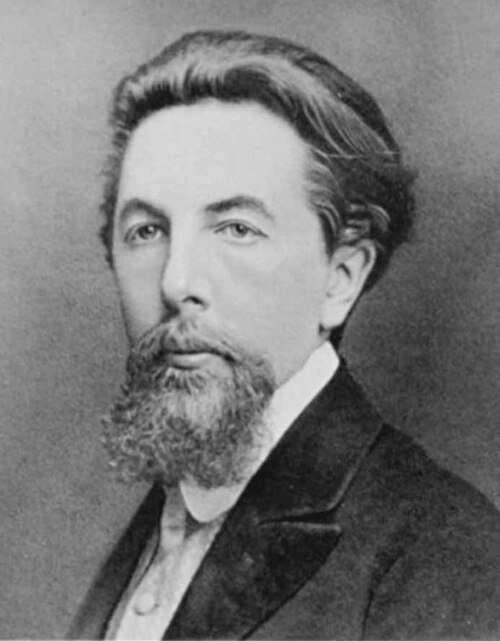
\includegraphics[width=\linewidth]{images/book3/tsvet.jpg}
\end{minipage}\hfill
\begin{minipage}[t]{0.78\linewidth}
\vspace{0pt}
Ahli botani Mikhail Tsvet menuangkan ekstrak daun hijau ke dalam tabung kaca
yang diisi serbuk kapur dan membilasnya dengan pelarut: pigmen-pigmennya
terpisah menjadi pita-pita berwarna, klorofil hijau dan karotenoid kuning.
Pada tahun 1906 ia menamai metode itu \omterm{def:b2:chromatography:principle}{kromatografi}, ``tulisan warna''.
Metode itu sebagian besar diabaikan selama seperempat abad, sampai
dipakai lagi untuk bahan alam pada tahun 1930-an. (Potret: pembuat tidak
diketahui, domain publik; Wikimedia Commons.)
\end{minipage}
\end{history}

\begin{safety}{\ghs[5mm]{GHS02}\,\ghs[5mm]{GHS05}\,\ghs[5mm]{GHS06}\,\ghs[5mm]{GHS07}\,\ghs[5mm]{GHS08}\,\ghs[5mm]{GHS09}}
Asetonitril dan metanol, komponen organik yang lazim dalam \omterm{def:b2:chromatography:principle}{fase gerak} HPLC,
mudah terbakar dan beracun; heksana, yang dipakai dalam \omterm{def:b2:chromatography:principle}{kromatografi} kolom,
mudah terbakar, membahayakan kesehatan, dan beracun bagi kehidupan akuatik.
Limbah pelarut dikumpulkan, tidak pernah dibuang ke wastafel.
% ledger: ghs:acetonitrile, ghs:methanol, ghs:hexane
\end{safety}

\section{Latihan}

\begin{exercise}[$\star$]\label{exo:b2:chromatography:1}
Sebuah senyawa mempunyai $t_R = \qty{5.0}{min}$ pada kolom yang \omterm{def:b2:chromatography:retention}{waktu matinya}
\qty{1.0}{min}. Hitunglah \omterm{def:b2:chromatography:retention}{faktor retensinya} dan fraksi waktunya yang
dihabiskan dalam \omterm{def:b2:chromatography:principle}{fase gerak}.
\end{exercise}

\begin{exercise}[$\star$]\label{exo:b2:chromatography:2}
Sebuah puncak pada $t_R = \qty{6.0}{min}$ mempunyai lebar dasar \qty{0.30}{min}. Hitunglah \omterm{def:b2:chromatography:plates}{bilangan pelatnya}.
\end{exercise}

\begin{exercise}[$\star$]\label{exo:b2:chromatography:3}
Sebuah kolom \qty{250}{mm} memberikan $N = 10\,000$ untuk sebuah senyawa. Hitunglah \omterm{def:b2:chromatography:plates}{tinggi pelatnya}.
\end{exercise}

\begin{exercise}[$\star$]\label{exo:b2:chromatography:4}
GC atau HPLC? Etanol dalam darah; sebuah protein; kafeina dalam minuman; benzena dalam bensin; gula dalam sari buah.
\end{exercise}

\begin{exercise}[$\star\star$]\label{exo:b2:chromatography:5}
Dua puncak: $t_{R1} = \qty{4.0}{min}$, $w_1 = \qty{0.40}{min}$; $t_{R2} = \qty{4.6}{min}$, $w_2 =
\qty{0.50}{min}$. Hitunglah \omterm{def:b2:chromatography:separation}{resolusinya}. Apakah keduanya terpisah sampai garis dasar?
\end{exercise}

\begin{exercise}[$\star\star$]\label{exo:b2:chromatography:6}
Berapa pelat yang diperlukan untuk memisahkan dua senyawa dengan $\alpha = 1.10$ dan $k_2 = 4.0$ pada
$R_s = 1.5$?
\end{exercise}

\begin{exercise}[$\star\star$]\label{exo:b2:chromatography:7}
Sebuah kolom mempunyai $A = \qty{5}{\micro m}$, $B = \qty{8}{\micro m.mm/s}$, $C = \qty{2}{\micro m.s/mm}$
(data latihan). Tentukan kecepatan optimum dan \omterm{def:b2:chromatography:plates}{tinggi pelat} terkecil.
\end{exercise}

\begin{exercise}[$\star\star$]\label{exo:b2:chromatography:8}
Ramalkan urutan \omterm{def:b2:chromatography:principle}{elusi} benzena, fenol, dan toluena dalam HPLC \omterm{def:b2:chromatography:techniques}{fase terbalik}
dengan \omterm{def:b2:chromatography:principle}{fase gerak} air--metanol, dan apa yang terjadi jika fraksi metanol
dinaikkan.
\end{exercise}

\begin{exercise}[$\star\star$]\label{exo:b2:chromatography:9}
Larutan kalibrasi sebuah analit pada \qty{20.0}{mg/L} dengan \omterm{def:b2:chromatography:quantitative}{standar internal}
pada \qty{10.0}{mg/L} memberikan luas 860 dan 400. Sampel yang ditambahi
standar pada \qty{10.0}{mg/L} memberikan luas 645 dan 410. Hitunglah \omterm{def:b2:chromatography:quantitative}{faktor
respons} dan konsentrasi analitnya (data latihan).
\end{exercise}

\begin{exercise}[$\star\star\star$]\label{exo:b2:chromatography:10}
Sebuah pemisahan memberikan $R_s = 1.06$. Panjang kolom berapakah,
relatif terhadap kolom yang sekarang, yang memberikan $R_s = 1.5$, dan
berapa biayanya dalam waktu? Tuas lain apa saja yang ada?
\end{exercise}

\begin{exercise}[$\star\star\star$]\label{exo:b2:chromatography:11}
Untuk dua puncak Gaussian dengan tinggi dan lebar yang sama dan lebar dasar
$w = 4\sigma$, hitunglah sinyal di tengah-tengah antara keduanya, relatif
terhadap tinggi puncak, pada $R_s = 1$ dan pada $R_s = 1.5$ (abaikan
sumbangan puncak yang jauh pada setiap maksimum).
\end{exercise}

\begin{exercise}[$\star\star\star$]\label{exo:b2:chromatography:12}
Pada $N$ dan $\alpha$ yang tetap, bandingkan faktor \omterm{def:b2:chromatography:separation}{resolusi} $k_2/(1+k_2)$
dan waktu analisis relatif $1 + k_2$ untuk $k_2 = 2$, 5, dan 10. Rentang $k$
manakah yang sebaiknya dipilih?
\end{exercise}

\section{Soal: Kafeina dalam Minuman Energi}

\begin{problem}[{Soal akhir pekan --- urutan elusi fase terbalik, kinerja
kolom dari sebuah kromatogram, memperbaiki pemisahan, dan kuantifikasi
dengan standar internal}]
\label{pb:b2:chromatography:1}
Data latihan (rekaan, bukan metode yang sebenarnya). Sebuah minuman energi
diencerkan sepuluh kali (\qty{5.00}{mL} menjadi
\qty{50.0}{mL}) dan teofilina ditambahkan sebagai \omterm{def:b2:chromatography:quantitative}{standar internal} pada
\qty{40.0}{mg/L} dalam larutan yang diencerkan. Kolom: \qty{150}{mm}, \omterm{def:b2:chromatography:techniques}{fase
terbalik}; \omterm{def:b2:chromatography:principle}{fase gerak} air--metanol; deteksi UV. Matriks yang tidak tertahan
(gula dan garam) terelusi pada $t_M = \qty{1.0}{min}$; teofilina pada
\qty{3.0}{min} (lebar dasar \qty{0.18}{min}); kafeina pada \qty{3.4}{min} (lebar dasar \qty{0.20}{min}).
Kalibrasi: kafeina \qty{50.0}{mg/L} dan teofilina \qty{40.0}{mg/L}
memberikan luas 1500 dan 1000. Sampel: luas 970 (kafeina) dan 1010
(teofilina). Sebuah kaleng berisi \qty{250}{mL}.
% ledger: ghs:caffeine, ghs:methanol

\begin{center}
\begin{tikzpicture}
\begin{axis}[width=0.75\linewidth, height=4.4cm, xmin=0, xmax=5, ymin=0, ymax=1,
  xlabel={waktu (min)}, ylabel={absorbans (s.b.)}, label style={font=\small},
  tick label style={font=\scriptsize}, ytick=\empty]
\addplot[omDef, thick] table[x=t, y=s] {figdata/out/bachelor-2-chromatogram-c.dat};
\node[font=\scriptsize] at (axis cs:1.0,0.42) {matriks};
\node[font=\scriptsize] at (axis cs:2.62,0.86) {teofilina};
\node[font=\scriptsize] at (axis cs:3.85,0.84) {kafeina};
\end{axis}
\end{tikzpicture}
\end{center}
% figdata: bachelor-2/chromatogram.py part c

\medskip
\noindent\textbf{Bagian I --- \omterm{def:b2:chromatography:techniques}{Fase terbalik}.}
\begin{enumerate}
  \item Uraikan \omterm{def:b2:chromatography:principle}{fase diam} dan \omterm{def:b2:chromatography:principle}{fase gerak} sebuah kolom \omterm{def:b2:chromatography:techniques}{fase terbalik}.
  \item Mengapa gula-gula terelusi pada \omterm{def:b2:chromatography:retention}{waktu mati}?
  \item Kafeina adalah 1,3,7-trimetilxantina, teofilina 1,3-dimetilxantina.
        Jelaskan urutan \omterm{def:b2:chromatography:principle}{elusinya}.
  \item Mengapa teofilina merupakan \omterm{def:b2:chromatography:quantitative}{standar internal} yang baik di sini?
  \item Apa yang akan terjadi pada kedua \omterm{def:b2:chromatography:retention}{waktu retensi} jika fraksi metanol dinaikkan?
  \item Apa yang diukur oleh \omterm{def:b2:chromatography:retention}{waktu mati}?
\end{enumerate}

\medskip
\noindent\textbf{Bagian II --- Kinerja kolom.}
\begin{enumerate}[resume]
  \item Hitunglah \omterm{def:b2:chromatography:retention}{faktor retensi} teofilina dan kafeina.
  \item Hitunglah \omterm{def:b2:chromatography:separation}{faktor selektivitasnya}.
  \item Hitunglah \omterm{def:b2:chromatography:plates}{bilangan pelat} untuk kafeina dan untuk teofilina.
  \item Hitunglah \omterm{def:b2:chromatography:plates}{tinggi pelat} untuk kafeina.
  \item Hitunglah \omterm{def:b2:chromatography:separation}{resolusi} di antara kedua puncak.
  \item Periksalah hasilnya dengan persamaan \omterm{def:b2:chromatography:separation}{resolusi}.
  \item Apakah puncak-puncak itu terpisah sampai garis dasar?
\end{enumerate}

\medskip
\noindent\textbf{Bagian III --- Lebih cepat atau lebih baik.}
\begin{enumerate}[resume]
  \item Untuk menghemat waktu, kolomnya dipendekkan menjadi \qty{75}{mm}
        (isian dan alir yang sama). Bagaimana \omterm{def:b2:chromatography:separation}{resolusinya}?
  \item Dan waktu analisisnya?
  \item Apa yang akan diberikan oleh kolom \qty{300}{mm} sebagai gantinya, dan dengan biaya apa?
  \item Tuas manakah yang bekerja pada $\alpha$?
  \item Apakah menaikkan $k$ akan banyak membantu di sini?
\end{enumerate}

\medskip
\noindent\textbf{Bagian IV --- Kuantifikasi.}
\begin{enumerate}[resume]
  \item Hitunglah \omterm{def:b2:chromatography:quantitative}{faktor respons} kafeina relatif terhadap teofilina.
  \item Mengapa volume suntikan tidak berpengaruh?
  \item Hitunglah konsentrasi kafeina dalam larutan yang diencerkan.
  \item Hitunglah konsentrasi kafeina dalam minuman itu.
  \item Apa yang akan salah jika sebuah senyawa matriks terelusi bersama teofilina?
  \item Apa yang akan diperlukan oleh kalibrasi eksternal sebagai gantinya?
  \item Nyatakan massa kafeina dalam sebuah kaleng \qty{250}{mL}.
\end{enumerate}
\end{problem}
